\documentclass{ctexart}

% === 关键:引入 standalone 包 ===
% 它的作用是:当主文件读取子文件时,会自动跳过子文件的 \documentclass 到 \begin{document} 之间的内容
\usepackage{standalone} 

% 设置章节格式 (ctexset 建议保留在 tex 文件里,或者也放进 sty)
\ctexset{
    section = {
        titleformat = \raggedright,
        name = {,、},
        number = \chinese{section}
    }
}

% === 引入公共配置 ===
\usepackage{template} 



\begin{document}

% 目录设置...
% 生成目录
% 设置目录格式

\renewcommand{\contentsname}{\centering\Huge\bfseries 目录}
\renewcommand{\cfttoctitlefont}{\hfill\Huge\bfseries}  % 目录标题字体
\renewcommand{\cftaftertoctitle}{\hfill\mbox{}}        % 确保标题居中
\renewcommand{\cftsecfont}{\Large\bfseries}            % 一级章节字体(增大)
\renewcommand{\cftsecpagefont}{\Large\bfseries}        % 一级章节页码字体(增大)
\renewcommand{\cftsubsecfont}{\large\bfseries}         % 二级章节字体(增大) 
\renewcommand{\cftsubsecpagefont}{\large\bfseries}     % 二级章节页码字体(增大)
\renewcommand{\cftsecdotsep}{\cftdotsep}               % 点状分隔符

% 调整目录间距
\setlength{\cftbeforesecskip}{25pt}                    % 增大章节间间距
\setlength{\cftbeforesubsecskip}{15pt}                 % 增大子章节间间距
\setlength{\cftaftertoctitleskip}{30pt}                % 增大目录标题后的间距

% 增加目录项之间的额外间距
\addtocontents{toc}{\setlength{\parskip}{7pt}}        % 段落间距
\addtocontents{toc}{\setlength{\itemsep}{5pt}}         % 项目间距
\tableofcontents
\thispagestyle{empty}  % 目录页不显示页脚

\newpage
\thispagestyle{empty}  % 空白页不显示页脚
\subsection*{}

\newpage
\setcounter{page}{1}  % 重置页码为1,从正文开始计算页码


% === 引入子文件 ===
% 注意:这里仍然使用 \input
\input{}
\newpage

\documentclass{ctexart} % 子文件也要声明类型

% === 引入公共配置 ===
% 这样单独编译时,它就有颜色和代码高亮了
\usepackage{my_style} 

\begin{document} 
% 注意:主文件读取时,会忽略上面的所有内容,直接从这里开始读取

\section{[CSP-J 2025] 座位 / seat} 

\subsection*{题目描述}
CSP-J 2025 第二轮正在进行。小 R 所在的考场共有 $n \times m$ 名考生,其中所有考生的 CSP-J 2025 第一轮成绩互不相同。所有 $n \times m$ 名考生将按照 CSP-J 2025 第一轮的成绩,由高到低蛇形分配座位,排列成 $n$ \textbf{行} $m$ \textbf{列}。具体地,设小 R 所在的考场的所有考生的成绩从高到低分别为 $s_1 > s_2 > \dots > s_{n \times m}$,则成绩为 $s_1$ 的考生的座位为第 1 \textbf{列}第 $1$ \textbf{行},成绩为 $s_2$ 的考生的座位为第 $1$ \textbf{列}第 $2$ \textbf{行},$\dots$,成绩为 $s_n$ 的考生的座位为第 $1$ \textbf{列}第 $n$ \textbf{行},成绩为 $s_{n+1}$ 的考生的座位为第 $2$ \textbf{列}第 $n$ \textbf{行},$\dots$,成绩为 $s_{2n}$ 的考生的座位为第 $2$ \textbf{列}第 $1$ \textbf{行},成绩为 $s_{2n+1}$ 的考生的座位为第 $3$ \textbf{列}第 $1$ \textbf{行},以此类推。

例如,若 $n = 4, m = 5$,则所有 $4 \times 5 = 20$ 名考生将按照 CSP-J 2025 第一轮成绩从高到低的顺序,根据下图中的箭头顺序分配座位。

\begin{figure}[h]
\centering
\includegraphics[width=0.6\textwidth]{image}
\caption{蛇形排列示意图($n=4, m=5$)}
\end{figure}

\subsection*{输入输出格式}
\textbf{输入:}第一行,两个正整数 $n, m$,分别表示考场座位的\textbf{行数}与\textbf{列数}。\par
\qquad\quad 第二行,$n \times m$ 个正整数 $a_1, a_2, \dots, a_{n \times m}$,表示所有考生 CSP-J 2025 第一轮的成绩,其中 $a_1$ 为小 R 的成绩。\par
\textbf{输出:}一行两个正整数 $c, r$,表示小 R 的座位为第 $c$ \textbf{列}第 $r$ \textbf{行}。

\begin{table}[h]
\centering
\begin{tabularx}{\textwidth}{|X|X|}
\hline
\textbf{输入示例} & \textbf{输出示例}     \\    
\hline
2 2 & 1 2   \\ 
99 100 97 98 & \\ 
\hline
2 2 & 2 2   \\ 
98 99 100 97 & \\ 
\hline
3 3 & 3 1   \\ 
94 95 96 97 98 99 100 93 92 & \\ 
\hline
\end{tabularx}  
\end{table}

\subsection*{样例解释}
\textbf{样例1:}成绩从高到低排序为:100, 99, 98, 97。

座位分配过程如下图所示:
\begin{figure}[h]
\centering
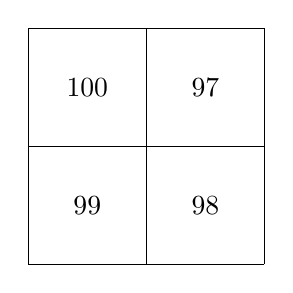
\begin{tikzpicture}[scale=1.5]
\draw (0,0) grid (2,2);
\node at (0.5,1.5) {100};
\node at (0.5,0.5) {99};
\node at (1.5,0.5) {98};
\node at (1.5,1.5) {97};
\end{tikzpicture}
\caption{样例1座位分配图(n=2, m=2)}
\end{figure}

小 R 的成绩为99,位于第1列第2行。

\textbf{样例2:}成绩从高到低排序为:100, 99, 98, 97。

座位分配与样例1相同,分配图如下:
\begin{figure}[h]
\centering
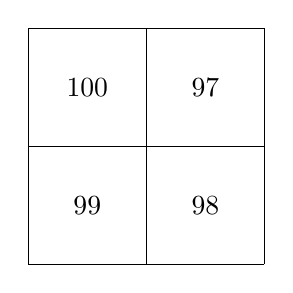
\begin{tikzpicture}[scale=1.5]
\draw (0,0) grid (2,2);
\node at (0.5,1.5) {100};
\node at (0.5,0.5) {99};
\node at (1.5,0.5) {98};
\node at (1.5,1.5) {97};
\end{tikzpicture}
\caption{样例2座位分配图(n=2, m=2)}
\end{figure}

但小 R 的成绩为98,因此座位为第2列第2行。

\subsection*{算法分析}
\begin{enumerate}
\item \textcolor{important}{\textbf{问题转化}}\\
本题的核心在于按照\textcolor{important}{\textbf{蛇形顺序}}填充矩阵,并找到目标成绩的坐标。首先,我们需要将所有考生的成绩\textcolor{important}{\textbf{从大到小排序}}。

\item \textcolor{important}{\textbf{规律观察}}\\
观察题目给出的蛇形排列方式,我们可以发现\textbf{列的奇偶性}决定了行的填充方向:
 \begin{enumerate}
    \item \textbf{奇数列(第1, 3, 5...列)}:成绩从\textcolor{important}{\textbf{上到下}}(行号 $1 \to n$)依次排列。
    \item \textbf{偶数列(第2, 4, 6...列)}:成绩从\textcolor{important}{\textbf{下到上}}(行号 $n \to 1$)依次排列。
 \end{enumerate}

\item \textcolor{important}{\textbf{算法步骤}}
 \begin{enumerate}
    \item 记录小 R 的原始成绩(输入数组的第一个数)。
    \item 对成绩数组进行降序排序。
    \item 使用一个全局指针 `idx` 指向排序后的成绩数组。
    \item \textcolor{important}{\textbf{外层循环}}枚举列号 $c$ 从 $1$ 到 $m$:
    \begin{itemize}
        \item 若 $c$ 为奇数,\textcolor{important}{\textbf{内层循环}}行号 $r$ 从 $1$ 到 $n$;
        \item 若 $c$ 为偶数,\textcolor{important}{\textbf{内层循环}}行号 $r$ 从 $n$ 到 $1$。
    \end{itemize}
    \item 在填充过程中,比较当前填入的成绩是否等于小 R 的成绩。若相等,立即输出当前的 $(c, r)$ 并结束程序。
 \end{enumerate}

\end{enumerate}

\subsection*{参考代码}
\begin{lstlisting}
#include "bits/stdc++.h"
using namespace std;
using u32 = unsigned;
using i32 = int;
using u64 = unsigned long long;
using i64 = long long;
using u128 = unsigned __int128;
using i128 = __int128;

#define int long long
#define endl "\n"

constexpr i64 inf = 1e18;

void slu() {
    int n, m;
    cin >> n >> m;
    vector<int> a(n * m);
    for (auto& x : a) cin >> x;
    int aim = a[0];
    sort(a.begin(), a.end(), greater());
    vector<vector<int>> M(n, vector<int>(m, 0));

    int x = 0, y = 0;
    int T = 0;
    int cur = 0;
    while (x < n && y < m) {
        M[x][y] = a[cur++];
        if (M[x][y] == aim) {
            cout << y + 1 << "` `" << x + 1;
            return;
        }
        if (T < n - 1) x++;
        else if (T == n - 1) y++;
        else if (T != 2 * n - 1) x--; 
        else y++;
        
        T = (T + 1) % (2 * n);
    }
}

signed main() {
    ios_base::sync_with_stdio(false);
    cin.tie(nullptr);
    cout.tie(nullptr);

    int t = 1;
    // cin >> t;

    while (t--) slu();
    return 0;
}
\end{lstlisting}

\subsection*{拓展思考}
\begin{itemize}
    \item \textcolor{important}{\textbf{数学推导($O(1)$ 解法)}}:
    假设小 R 的成绩在排序后排在第 $k$ 名(下标从 0 开始)。
    \begin{enumerate}
        \item 所在的列号:$c = k / n + 1$。
        \item 所在的行号:
        \begin{itemize}
            \item 若 $c$ 为奇数,行号 $r = (k \% n) + 1$;
            \item 若 $c$ 为偶数,行号 $r = n - (k \% n)$。
        \end{itemize}
    \end{enumerate}
    这种方法无需模拟整个矩阵,效率更高。
    \begin{lstlisting}
int n, m;
cin >> n >> m;
vector<int> a(n *m);
for (auto &x : a) cin >> x;

int target = a[0];
sort(a.begin(), a.end(), greater<int>());

int idx = -1;
for (int i = 0; i < n * m; i++) {
    if (a[i] == target) {
        idx = i;
        break;
    }
}

int c = idx / n + 1;
int r;
if (c % 2 != 0) {
    r = (idx % n) + 1;
} else {
    r = n - (idx % n);
}

cout << c << "` `" << r << endl;
    \end{lstlisting}
\end{itemize}

\end{document}
\newpage

\documentclass{ctexart} % 子文件也要声明类型

% === 引入公共配置 ===
% 这样单独编译时,它就有颜色和代码高亮了
\usepackage{my_style} 

\begin{document} 
% 注意:主文件读取时,会忽略上面的所有内容,直接从这里开始读取

\section{[CSP-J 2025] 异或和 / xor} 

\subsection*{题目描述}
小 R 有一个长度为 $n$ 的非负整数序列 $a_1, a_2, \dots, a_n$。定义一个区间 $[l, r]$ ($1 \leq l \leq r \leq n$) 的权值为 $a_l, a_{l+1}, \dots, a_r$ 的二进制按位异或和,即 $a_l \oplus a_{l+1} \oplus \dots \oplus a_r$,其中 $\oplus$ 表示二进制按位异或。

小 X 给了小 R 一个非负整数 $k$。小 X 希望小 R 选择序列中尽可能多的不相交的区间,使得每个区间的权值均为 $k$。两个区间 $[l_1, r_1], [l_2, r_2]$ 相交当且仅当两个区间同时包含至少一个相同的下标,即存在 $1 \leq i \leq n$ 使得 $l_1 \leq i \leq r_1$ 且 $l_2 \leq i \leq r_2$。

例如,对于序列 $[2, 1, 0, 3]$,若 $k = 2$,则小 R 可以选择区间 $[1, 1]$ 和区间 $[2, 4]$,权值分别为 $2$ 和 $1 \oplus 0 \oplus 3 = 2$;若 $k = 3$,则小 R 可以选择区间 $[1, 2]$ 和区间 $[4, 4]$,权值分别为 $1 \oplus 2 = 3$ 和 $3$。

\subsection*{输入输出格式}
\textbf{输入:}第一行,两个非负整数 $n, k$,分别表示序列长度和给定的非负整数。\par
\qquad\quad 第二行,$n$ 个非负整数 $a_1, a_2, \dots, a_n$,表示小 R 的序列。\par
\textbf{输出:}一行一个非负整数,表示能选出的不相交区间数量的最大值。

\begin{table}[h]
\centering
\begin{tabularx}{\textwidth}{|X|X|}
\hline
\textbf{输入示例} & \textbf{输出示例}     \\    
\hline
4 2 & 2   \\ 
2 1 0 3 & \\ 
\hline
4 3 & 2   \\ 
2 1 0 3 & \\ 
\hline
4 0 & 1   \\ 
2 1 0 3 & \\ 
\hline
\end{tabularx}  
\end{table}

\subsection*{样例解释}
\textbf{样例1:}可以选择区间 $[1, 1]$ 和区间 $[2, 4]$,异或和分别为 $2$ 和 $1 \oplus 0 \oplus 3 = 2$,且两个区间不相交。

\textbf{样例2:}可以选择区间 $[1, 2]$ 和区间 $[4, 4]$,异或和分别为 $1 \oplus 2 = 3$ 和 $3$,且两个区间不相交。

\textbf{样例3:}可以选择区间 $[3, 3]$,异或和为 $0$。不能同时选择区间 $[3, 3]$ 和区间 $[1, 4]$,因为这两个区间相交。

\subsection*{算法分析}
\begin{enumerate}
\item \textcolor{important}{\textbf{前缀异或性质}}\\
定义 $pre[i]$ 为序列前 $i$ 个元素的异或和(即 $a_1 \oplus a_2 \oplus \dots \oplus a_i$),规定 $pre[0] = 0$。
根据异或的性质,任意区间 $[l, r]$ 的异或和可以表示为:
$$a_l \oplus \dots \oplus a_r = pre[r] \oplus pre[l-1]$$
题目要求区间异或和为 $k$,即 $pre[r] \oplus pre[l-1] = k$,移项得:
\textcolor{important}{$$pre[l-1] = pre[r] \oplus k$$}

\item \textcolor{important}{\textbf{动态规划状态定义}}\\
设 $dp[i]$ 表示在序列的前 $i$ 个数中,能够选出的满足条件的不相交区间的\textbf{最大数量}。

\item \textcolor{important}{\textbf{状态转移方程}}\\
对于当前位置 $i$,我们有两种选择策略:
\begin{enumerate}
    \item \textbf{不以 $i$ 作为区间的结尾}:此时最大数量继承自前一个位置,即 $dp[i] = dp[i-1]$。
    \item \textbf{寻找一个区间以 $i$ 结尾}:我们需要找到一个下标 $j$ ($0 \le j < i$),使得区间 $[j+1, i]$ 的异或和为 $k$。
    \begin{itemize}
        \item 由前缀异或性质可知,需要满足 $pre[j] = pre[i] \oplus k$。
        \item 如果存在这样的 $j$,则可以转移:$dp[i] = \max(dp[i], dp[j] + 1)$。
    \end{itemize}
\end{enumerate}
综上,状态转移方程为:
$$dp[i] = \max(dp[i-1], \max_{j \text{ satisfying condition}} (dp[j] + 1))$$

\item \textcolor{important}{\textbf{哈希表优化}}\\
为了快速找到满足 $pre[j] = pre[i] \oplus k$ 
的最佳下标 $j$,我们使用哈希表 map$<$int, int$>$

\begin{itemize}
    \item \textbf{键 (Key)}:前缀异或值 $val$。
    \item \textbf{值 (Value)}:该前缀异或值对应的下标 $j$。
    \item \textbf{贪心更新策略}:为了保证 $dp[i]$ 最大,我们在哈希表中记录该前缀异或值出现时对应的\textbf{最大 $dp$ 值}的下标。即:当计算出新的 $dp[i]$ 后,如果它比之前记录的同前缀异或值的 $dp$ 结果更优,才更新哈希表。
\end{itemize}

\end{enumerate}

\subsection*{参考代码}
\begin{lstlisting}
#include "bits/stdc++.h"
using namespace std;

using u32 = unsigned;
using i32 = int;
using u64 = unsigned long long;
using i64 = long long;
using u128 = unsigned __int128;
using i128 = __int128;

#define int long long
#define endl "\n"

constexpr i64 inf = 1e18;

void slu() {
    int n, k;
    cin >> n >> k;
    vector<int> a(n);
    for (auto &x : a) cin >> x;
    vector<int> pre(n + 1, 0);
    map<int, int> mp;
    vector<int> dp(n + 1, 0);
    for (int i = 1; i <= n; i++) {
        pre[i] = pre[i - 1] ^ a[i - 1];
    }

    mp[0] = 0;
    for (int i = 1; i <= n; i++) {
        int l = pre[i] ^ k;
        dp[i] = dp[i - 1];
        if (mp.contains(l)) {
            dp[i] = max(dp[i], dp[mp[l]] + 1);
        }
        if (dp[i] > dp[mp[pre[i]]]) {
            mp[pre[i]] = i;
        }
    }
    cout << dp[n];
}

signed main() {
    ios_base::sync_with_stdio(false);
    cin.tie(nullptr);
    cout.tie(nullptr);

    int t = 1;
    // cin >> t;

    while (t--) slu();
    return 0;
}

\end{lstlisting}

\subsection*{拓展思考}
\begin{itemize}
    \item \textcolor{important}{\textbf{优化空间}}:可以使用 \texttt{unordered\_map} 替代 \texttt{map},将单次查找的时间复杂度从 $O(\log n)$ 优化到期望 $O(1)$,从而将总时间复杂度优化到 $O(n)$。
\end{itemize}

\end{document}
% 主文件读取到这里就会停止 
\newpage

\documentclass{ctexart} % 子文件也要声明类型

% === 引入公共配置 ===
% 这样单独编译时,它就有颜色和代码高亮了
\usepackage{my_style} 

\begin{document} 
% 注意:主文件读取时,会忽略上面的所有内容,直接从这里开始读取




\section{[CSP-J 2025] 多边形 / polygon} 

\subsection*{题目描述}
小 R 有 $n$ 根小木棍,第 $i$ ($1 \leq i \leq n$) 根小木棍的长度为 $a_i$。小 X 希望小 R 从这 $n$ 根小木棍中选出若干根小木棍,将它们按任意顺序首尾相连拼成一个多边形。拼成多边形的条件:对于长度分别为 $l_1, l_2, \dots, l_m$ 的 $m$ 根小木棍,能拼成一个多边形当且仅当 $m \geq 3$ 且所有小木棍的长度之和大于所有小木棍的长度最大值的两倍,即 $\sum_{i=1}^{m} l_i > 2 \times \max_{i=1}^{m} l_i$。

小 X 提出的问题是:有多少种选择小木棍的方案,使得选出的小木棍能够拼成一个多边形?两种方案不同当且仅当选择的小木棍的下标集合不同。由于答案可能较大,你只需要求出答案对 $998,244,353$ 取模后的结果。

\subsection*{输入输出格式}
\textbf{输入:}第一行,一个正整数 $n$,表示小木棍的数量。\par
\qquad\quad 第二行,$n$ 个正整数 $a_1, a_2, \dots, a_n$,表示小木棍的长度。\par
\textbf{输出:}一行一个非负整数,表示能拼成多边形的方案数对 $998,244,353$ 取模后的结果。

\begin{table}[h]
\centering
\begin{tabularx}{\textwidth}{|X|X|}
\hline
\textbf{输入示例} & \textbf{输出示例}     \\    
\hline
5 & 9   \\ 
1 2 3 4 5 & \\ 
\hline
5 & 6   \\ 
2 2 3 8 10 & \\ 
\hline
\end{tabularx}  
\end{table}

\subsection*{样例解释}
\textbf{样例1:}共有9种选择方案能使选出的小木棍拼成多边形,具体方案如下:

\begin{enumerate}
\item 选择第 2,3,4 根小木棍,长度之和为 $2+3+4=9$,满足 $9 > 2 \times 4 = 8$;
\item 选择第 2,4,5 根小木棍,长度之和为 $2+4+5=11$,满足 $11 > 2 \times 5 = 10$;
\item 选择第 3,4,5 根小木棍,长度之和为 $3+4+5=12$,满足 $12 > 2 \times 5 = 10$;
\item 选择第 1,2,3,4 根小木棍,长度之和为 $1+2+3+4=10$,满足 $10 > 2 \times 4 = 8$;
\item 选择第 1,2,3,4,5 根小木棍,长度之和为 $1+2+3+4+5=15$,满足 $15 > 2 \times 5 = 10$。
\item \dots
\end{enumerate}

\subsection*{算法分析}
\begin{enumerate}
\item \textcolor{important}{\textbf{问题转化与补集思想}}\\
直接计算合法方案较为困难,我们采用\textcolor{important}{\textbf{正难则反}}的策略。
\begin{itemize}
    \item \textbf{总方案数推导}:
    对于 $n$ 根木棍,每一根木棍都有“选”或“不选”两种状态。根据数学中的乘法原理,
    总的组合数为 $2 \times 2 \times \dots \times 2 = 2^n$ 种。
    由于题目要求选出木棍(空集没有意义),我们扣除掉“一根都不选”的情况,
    因此总方案数 : $$ Total = 2^n - 1$$
    \item \textbf{合法条件}:集合总和 $Sum > 2 \times Max$。
    \item \textbf{非法条件}:集合总和 $Sum \leq 2 \times Max$。
    \item 设集合中除最大值以外的元素和为 $S_{rest}$,则非法条件等价于:
    \[ S_{rest} + Max \leq 2 \times Max \implies \textcolor{important}{S_{rest} \leq Max} \]
    \item \textbf{结论}:若除最大边外的其余边之和不超过最大边,则该集合无法构成多边形。
\end{itemize}

\item \textcolor{important}{\textbf{排序与枚举}}
 \begin{enumerate}
    \item 首先将数组 $a$ 从小到大\textcolor{important}{\textbf{排序}}。
    \item 枚举每一个 $a_i$ 作为当前子集的\textbf{最大值}。
    \item 此时,我们只能从下标 $[0, i-1]$ 的木棍中选择若干根,使得它们的和 $\leq a_i$。这些组合即为以 $a_i$ 为最大值的\textbf{非法方案}。
 \end{enumerate}

\item \textcolor{important}{\textbf{动态规划(01背包)}}
\begin{itemize}
    \item \textbf{定义}:$dp[j]$ 表示从之前的木棍中选出若干根,长度之和为 $j$ 的方案数。
    \item \textbf{非法统计}:对于当前的 $a_i$,
    所有满足 $j \leq a_i$ 的 $dp[j]$ 之和,即为以 $a_i$ 为最大值的非法方案数。
\begin{lstlisting}
for (int j = 0; j <= a[i]; j++) {
    illegal = (illegal + dp[j]) % MOD;
}
\end{lstlisting}

    \item \textbf{转移}:统计完成后,
    将 $a_i$ 加入背包供后续使用(01背包倒序更新):$dp[j] = dp[j] + dp[j - a_i]$。
\begin{lstlisting}
for (int j = Max; j >= a[i]; j--) {
    dp[j] = (dp[j] + dp[j - a[i]]) % MOD;
}
\end{lstlisting}

    \item \textbf{最终答案}:
    $Total - Illegal = (2^n - 1) - 
    \sum (\text{针对每个 } a_i \text{ 的非法方案})$。
\end{itemize}

\end{enumerate}

\subsection*{算法复杂度分析}
\begin{itemize}
    \item \textcolor{important}{\textbf{时间复杂度}}:$O(n \times V)$,其中 $V = \max(a_i)$。我们需要遍历 $n$ 个元素,对于每个元素,都需要更新大小为 $V$ 的背包数组。
    \item \textcolor{important}{\textbf{空间复杂度}}:$O(V)$,其中 $V = \max(a_i)$,用于存储动态规划数组 $dp$。
\end{itemize}

\subsection*{代码实现}
\begin{lstlisting}
#include <bits/stdc++.h>
using namespace std;
using i64 = long long;
#define int long long
constexpr i64 inf = 1e18;
constexpr i64 MOD = 998244353;

int qpow(int a, int b, int m) {
    a %= m;
    int res = 1;
    while (b > 0) {
        if (b & 1) res = res * a % m;
        a = a * a % m;
        b >>= 1;
    }
    return res % m;
}

void slu() {
    int n;
    cin >> n;
    vector<int> a(n);
    for (int i = 0; i < n; i++) cin >> a[i];
    sort(a.begin(), a.end());

    int Max = a.back(),illegal = 0;
    int res = qpow(2, n, MOD) - 1;
    vector<int> dp(Max + 1, 0);
    dp[0] = 1;

    for (int i = 0; i < n; i++) {
        for (int j = 0; j <= a[i]; j++) {
            illegal = (illegal + dp[j]) % MOD;
        }
        for (int j = Max; j >= a[i]; j--) {
            dp[j] = (dp[j] + dp[j - a[i]]) % MOD;
        }
    }
    res = (res - illegal + MOD) % MOD;
    cout << res << endl;
}

signed main() {
    ios_base::sync_with_stdio(false);cin.tie(nullptr);
    slu();
    return 0;
}

\end{lstlisting}



\end{document}
\newpage
\end{document}